% chktex-file 8
% chktex-file 44
% chktex-file 17
% chktex-file 36
% chktex-file 13
% chktex-file 15
%chktex-file 16
%chktex-file 39
\documentclass[12pt,a4paper,english]{article}
\usepackage[utf8]{inputenc}
\usepackage[british]{babel}

%%MUST STAY HERE
\usepackage[svgnames, table]{xcolor}
%%

\usepackage{amsfonts}
\usepackage{amsthm}
\usepackage{amsmath}
\usepackage{array}
\usepackage{amssymb}
\usepackage{arydshln}
\usepackage{attachfile}

\usepackage{booktabs}
\usepackage[some]{background}

\usepackage{dsfont}

\usepackage{eurosym}
\usepackage[euler-digits]{eulervm}

\usepackage{fancyhdr}
\usepackage[T1]{fontenc}
\usepackage{fullpage}
\usepackage{fontspec} %requires compilation via lualatex
\usepackage{graphicx}

\usepackage{hyperref}
%%Must stay here
\usepackage{caption}
\usepackage{cleveref}
%%
\usepackage{hhline}

\usepackage{mathtools}
\usepackage{minted}
\usepackage{multicol}
\usepackage{multirow}

\usepackage[numbers,sort]{natbib}
\usepackage{navigator}

\usepackage{pageslts}
\usepackage{palatino}
\usepackage{pifont}
\usepackage{pgffor}
\usepackage{pgfplots}

\usepackage{siunitx}

\usepackage{tabularx}
\usepackage{tikz}

\usepackage{verbatim}

%\usepackage{xwatermark}
%%Fonts%%
\defaultfontfeatures{Mapping=tex-text}
\setmainfont%
[Mapping=tex-text, Color=black,
%BoldFont=DroidSerif-Bold.ttf,
%ItalicFont=DroidSerif-Italic.ttf,
%BoldItalicFont=DroidSerif-BoldItalic.ttf
BoldFont=CormorantGaramond-SemiBold.otf,
ItalicFont=CormorantGaramond-LightItalic.otf,
BoldItalicFont=CormorantGaramond-MediumItalic.otf,
SmallCapsFont=CormorantSC-Regular.otf
]
{CormorantGaramond-Medium.otf}
\setmonofont{SourceCodePro-Regular.otf}[Scale=MatchLowercase]

%{DroidSerif-Regular.ttf}

%\setmathfont{texgyreheros-regular.otf}

%%Watermark
\backgroundsetup{
scale=10,
color=gray!20,
angle=45,
opacity=1,
contents= {Watermarking}
}

\captionsetup[figure]{labelfont={bf, it},textfont={it}}

%%%New commands%%%
\newcommand{\cmark}{\ding{51}}%
\newcommand{\xmark}{\ding{55}}%
\renewcommand{\arraystretch}{1.2}

\pagestyle{fancy} 
\fancyhf{}
\renewcommand{\headrulewidth}{0pt}

\definecolor{gblue}{HTML}{3366CC}
\definecolor{gred}{HTML}{DC3912}
\definecolor{gyellow}{HTML}{FF9900}
\definecolor{ggreen}{HTML}{109618}
\definecolor{gpurple}{HTML}{990099}
\definecolor{gseablue}{HTML}{0099C6}
\definecolor{gpastelpink}{HTML}{DD4477}


\pgfplotsset{compat=1.16}
\pgfplotsset{every axis/.append style={
  legend pos=north east,
  grid=major,
  major grid style={line width=.2pt, draw=black, dotted},
  axis x line=bottom,
  axis y line=left,
  no marks,
  axis line style=-,
  scaled y ticks=false,
  log basis x=2,
  log basis y=2,
  cycle list={
    {draw=gblue,thick},
    {densely dashed,draw=gred,thick},
    {loosely dashed,draw=gyellow,thick},
    {dashdotted,draw=ggreen,thick},
    {densely dotted,draw=gpurple,thick},
    {loosely dashdotted,draw=gseablue,thick},
  }
}}


\usetikzlibrary{spy,backgrounds}


\hypersetup{
  pdfborder = {0 0 0}
}

\newtheoremstyle{thm}% name of the style to be used
  {3pt}% measure of space to leave above the theorem. E.g.: 3pt
  {3pt}% measure of space to leave below the theorem. E.g.: 3pt
  {\itshape}% name of font to use in the body of the theorem
  {0pt}% measure of space to indent
  {\bfseries}% name of head font
  {}% punctuation between head and body
  { }% space after theorem head; " " = normal interword space
  {\thmname{#1}\thmnumber{ #2} \thmnote{\bf (#3)}\\}% Manually specify head
  
\newtheoremstyle{def}% name of the style to be used
  {3pt}% measure of space to leave above the theorem. E.g.: 3pt
  {3pt}% measure of space to leave below the theorem. E.g.: 3pt
  {\normalfont}% name of font to use in the body of the theorem
  {0pt}% measure of space to indent
  {\bfseries}% name of head font
  {}% punctuation between head and body
  { }% space after theorem head; " " = normal interword space
  {\thmname{#1}\thmnumber{ #2} \thmnote{\bf (#3)}\\}% Manually specify head
  
%\newcommand\stareq{\stackrel{\mathclap{\normalfont\mbox{*}}}{=}}
\renewcommand{\thefootnote}{\fnsymbol{footnote}}

\makeatletter
\newcommand{\oset}[3][0ex]{%
  \mathrel{\mathop{#3}\limits^{
    \vbox~to#1{\kern-2\ex@%
    \hbox{$\scriptstyle#2$}\vss}}}}
\makeatother

%\theoremstyle{thm}
\newtheorem{theorem}{Theorem}[section]
\newtheorem{lemma}[theorem]{Lemma}
\newtheorem{proposition}[theorem]{Proposition}
\newtheorem{corollary}[theorem]{Corollary}
\newtheorem{property}[theorem]{Propriety}
%\theoremstyle{def}
\newtheorem{definition}{Definition}[section]

\usetikzlibrary{calc}
\usetikzlibrary{shapes,arrows,arrows.meta}
\usetikzlibrary{automata,positioning}

\newcommand{\overtilde}[1]{\mathpalette\overtildex{#1}}
\newcommand{\overtildesym}{\sim}
%\makeatletter
\newcommand{\overtildex}[2]{
  \ifx\displaystyle#1\oset[-0.95ex]{\overtildesym}{#2\vphantom{i}}\fi
  \ifx\textstyle#1\oset[-.7ex]{\overtildesym}{#2\vphantom{i}}\fi
  \ifx\scriptstyle#1\oset[-.6ex]{\overtildesym}{#2\vphantom{i}}\fi
  \ifx\scriptscriptstyle#1\oset[-.3ex]{\overtildesym}{#2\vphantom{i}}\fi
}
%\makeatother

%%%%%%%%%%%%%%%%%%%%%%%%%%%%%%%%%%%%%%%%%%%%%%%%%%%%%%%%%%%%%%%%%%%%%%%%%%%%%%%%%%

\begin{document}

\pagenumbering{arabic}
\rfoot{Image Watermarking \thepage\ of \lastpageref{pagesLTS.arabic}}

\begin{titlepage}
  \BgThispage%
\begin{center}
\vspace{3cm}

\Large

\vspace{2cm}

\includegraphics[scale=0.25]{Cherubino.jpg}

  \vspace{2cm}
  {\sc \Huge A parallel solution}

  {\sc \Huge for image watermarking}

  {\Large Gemma Martini}
  \vspace{1.5cm}

  {\Large \sc Parallel and Distributed Systems}

  {\Large \sc Paradigms and Principles}

  \vspace{0.25cm}

{\Large \sc a.y. 2017-2018}

  \vspace{0.5cm}
  \abstract{
 The task of image watermarking consists in operating on any single pixel of an image, in order to add a background effect to that image.

In the real World, such a technique is performed to ``embed'' the ownership of a logo or a template, a toy example of a watermark is displayed in this page.

In this paper, we studied how to parallelize the computation of watermarking a set of images, starting from a theoretical model and then digging into the technical details of the implementation.
  }

\vfill
\centering

  \vspace{0.25cm}
  {\large \today}

\end{center}
\end{titlepage}

%%%%%%%%%%%%%%%%%%%~~~~~~~~~~~~~~~~~~~~~~~~~~~~~~~~~~~~~~~~~~~%%%%%%%%%%%%%%%%%%%%%%

\tableofcontents
\thispagestyle{empty}
\newpage
\setcounter{page}{1}

\renewcommand{\U}{l}
\newcommand{\I}{h}
\newcommand{\Bkind}[1]{B#1}
\newcommand{\Bn}{\Bkind{N}(\cal{N})}
\newcommand{\Br}{\Bkind{R}}
\newcommand{\Bd}{\Bkind{D}}

%%%%%%%%%%%%%%~~~~~~~~~~~~~~~~~~~~~~~~~~~~~~~~~~~~~~~~%%%%%%%%%%%%%%%
\section{Introduction}\label{intro}
%%%%%%%%%%%%%%~~~~~~~~~~~~~~~~~~~~~~~~~~~~~~~~~~~~~~~~%%%%%%%%%%%%%%
The watermarking problem was attacked preparing a vast set of black and white images as watermarks and a huge set of images to be watermarked.

Each pixel of the image which corresponds to a black pixel in the watermark needs to be updated.

We are going to show that this time is quite smaller than the time needed for loading and storing a picture, hence in this paper we also address a similar problem, which is a simplification of the original one: only one image gets watermarked and it is not stored on disk, after the operation. The strategy is to copy in main memory that specific image several times and the apply the watermark to each of them, accordingly to different algorithms.

\begin{comment}
The aim of this brief report is to show the project choices in creating a sequential and parallel tool that adds a watermark to a set of pictures. Implementation choices were made prioritizing the realistic case in which the watermark has a small fraction of black pixels, but results are reported covering most cases.

The folders that contain the surce images have the names FewImgs, MedImgs and Imgs and may be found in the home of the author (spm2018-martini). The folder WMSmall contains some kinds of watermark and can be found in the home of the author as well. In particular, watermarks {\tt blotches-01.png} and {\tt random-05.png} are the ones the algorithm is optimized for.

The folder containing the projects is made of several files, here is a list:
\begin{description}
  \item[\tt CImg.h] is the header of the library used to process imges;
  \item[\tt experiments.sh] is the script to run the experiments on the different images and watermarks and parallelism degree;
  \item[\tt Makefile] contains all the targets and should be called to compile;
  \item[\tt watermark1.0.cpp] is the source code of the sequential version, see \Cref{algo} for details;
 \item[\tt watermark2.0.cpp] is the source code obtained using OpenMP, see \Cref{2.0} for details;
 \item[\tt watermark2.1.cpp] is still parallel and obtained with OpenMP, but used in a different context, as explained in \Cref{2.1}
 \item[\tt watermark3.0.cpp] is the source code of a parallel implementation obtained using C++ threads. This implementation is focused in \Cref{3.0};
 \item[\tt watermark4.0.cpp] is the source code written using the C++ library FastFlow, for more details see \Cref{4.0};
  \item[\tt watermark1.0, watermark2.0, watermark2.1, watermark3.0 and watermark4.0] are the executables from the source code described above and have been compiled on the Xeon Phi.
\end{description}

\end{comment}

%%%%%%%%%%%%%%~~~~~~~~~~~~~~~~~~~~~~~~~~~~~~~~~~~~~~~~%%%%%%%%%%%%%%%
\section{A theoretical analysis}\label{sec:theoretical}
%%%%%%%%%%%%%%~~~~~~~~~~~~~~~~~~~~~~~~~~~~~~~~~~~~~~~~%%%%%%%%%%%%%%
The problem of image watermarking can be explained decomposing it into $4$ main operations. At first, the \emph{watermark} needs to be \emph{loaded} in main memory from disk; once this operation has been performed, we may proceed \emph{loading} the \emph{first image} to be watermarked, then it is \emph{modified} and \emph{stored}, until all the input images have been successfully watermarked.

Before digging into technicalities, we want to focus the attention of the reader on two main issues of this approach: first, we did not take into account any operation that allows us to keep track of which image has been processed and which are the ones that still need to be watermarked. On the other hand, this naıve approach, makes use of many unecessary conditional clauses in order to check whether the current pixel of the watermark is black (hence the image should be modified).

An attentive reader may notice at this point that two simple edits may be performed to overcome this issues. We add \emph{two} intermediate \emph{phases} between the operation of loading the watermark in memory and the load of the first image: we \emph{process the watermark} in order to store only the positions of the black pixels and we \emph{identify the input images} by means of a list.

A pictorial representation of such a solution is displayed in \Cref{fig:sequential}.

\begin{figure}[h]
\begin{center}
  \begin{tikzpicture}
    \tikzset{nd/.style={
      cloud,
      draw,
      cloud puffs=30,
      cloud puff arc=120,
      aspect=1.2,
      inner ysep=.3em,
      align=center}}
    \node[nd] at (0, 0) (0) {Load \\ wm};
    \node[nd] at (2.5, 0) (1) {Process \\ wm};
    \node[nd] at (5.5, 0) (2) {Process \\ imageList};
    \node at (8, 0) [rectangle,draw,align=center] (3) {Load\\image};
    \node at (10, 0) [rectangle,draw,align=center] (4) {Edit\\ image};
    \node at (12, 0) [rectangle,draw,align=center] (5) {Store\\ image};
    \draw[->] (0) -- (1);
    \draw[->] (1) -- (2);
    \draw[->] (2) -- (3);
    \draw[->] (3) -- (4);
    \draw[->] (4) -- (5);
    \draw [decorate,decoration={brace,amplitude=10pt,mirror,raise=20pt}] (3.west) -- (5.east) node [black,midway,yshift=-1.4cm] {\footnotesize $n$ times};
  \end{tikzpicture}
  \caption{The curly tasks are of a sequential nature and concur to the value of the serial fraction, while the rectangular tasks can be parallelized.}\label{fig:sequential}
\end{center}
\end{figure}

where $n$ is the number of input images to be watermarked.

Notice that in this problem the \emph{serial fraction} is represented as the time spent to execute the three ``cloudy'' operation over the total cost of all the $3 \cdot n + 3$ operations. Formally,

\[
  f = \frac{t_{\text{load wm}} + t_{\text{process wm}} + t_{\text{process imgList}}}{t_{\text{load wm}} + t_{\text{process wm}} + t_{\text{process imgList}} + n \cdot (t_{\text{load}} + t_{\text{edit}} + t_{\text{store}})}
\]

In this context the expected speedup using $n_w$ workers is computed as follows

\[
  sp(n_w) = \frac{t_{\text{seq}}}{f \cdot t_{\text{seq}} + \frac{(1-f) \cdot t_{\text{seq}}}{n_w}}
\]

Thanks to Gustaffson law we would expect the serial fraction to be amoritized when the data grain becomes finer and finer (the amount of data to be processed increases).

Let us analyze some parallel executions of such stages.

Since we are in presence of embarassing parallelism, we start by introducing the \emph{map} pattern on this problem.

\begin{figure}[h]
\begin{center}
  \begin{tikzpicture}
    \tikzset{nd/.style={
      cloud,
      draw,
      cloud puffs=30,
      cloud puff arc=120,
      aspect=1.2,
      inner ysep=.3em,
      align=center}}
    \node[nd] at (0, 0) (0) {Load \\ wm};
    \node[nd] at (2.5, 0) (1) {Process \\ wm};
    \node[nd] at (5.5, 0) (2) {Process \\ imageList};
    \node at (8, -2) [rectangle,draw,align=center] (3) {Load\\image};
    \node at (10, -2) [rectangle,draw,align=center] (4) {Edit\\ image};
    \node at (12, -2) [rectangle,draw,align=center] (5) {Store\\ image};
    \node at (10, 0) [align=center] (9) {\vdots};

    \node at (8, 2) [rectangle,draw,align=center] (6) {Load\\image};
    \node at (10, 2) [rectangle,draw,align=center] (7) {Edit\\ image};
    \node at (12, 2) [rectangle,draw,align=center] (8) {Store\\ image};

    \draw[->] (0) -- (1);
    \draw[->] (1) -- (2);
    \draw[->] (2) -- (3.west);
    \draw[->] (3) -- (4);
    \draw[->] (4) -- (5);
    \draw[->] (2) -- (6.west);
    \draw[->] (6) -- (7);
    \draw[->] (7) -- (8);

    \draw [decorate,decoration={brace,amplitude=10pt,mirror,raise=20pt}] (3.west) -- (5.east) node [black,midway,yshift=-1.4cm] {\footnotesize $\frac{n}{n_w}$ times};
    \draw [decorate,decoration={brace,amplitude=10pt,mirror,raise=30pt}] (5.south) -- (8.north) node [black,midway,xshift=1.8cm] {\footnotesize $n_w$};
  \end{tikzpicture}
  \caption{The tasks representd as curly circles cannot be parallelized, while the ones represented by squares can be (and are) parallelized.}\label{fig:data_parallel}
\end{center}
\end{figure}

In \Cref{fig:data_parallel} a pictorial representation of what can be formalized as 

\noindent \texttt{{\bf pipe}(load wm, process wm, process imglist, {\bf map}($n_w$, load img, edit img, store img))}.

On the other hand, this computation may be studied from another point of view using \emph{stream parallelism}, as presented \Cref{fig:stream_parallel}.

\begin{figure}[h]
  \centering
  \begin{tikzpicture}
    \tikzset{nd/.style={
      cloud,
      draw,
      cloud puffs=30,
      cloud puff arc=120,
      aspect=1.2,
      inner ysep=.3em,
      align=center}}
    \begin{scope}[scale=1, xshift=5mm, yshift=2.5cm]
    \node[nd] at (0, 0) (0) {Load \\ wm};
    \node[nd] at (2.3, 0) (1) {Process \\ wm};
    \node[nd] at (5, 0) (2) {Process \\ imageList};
    \node at (7.3, 0) [circle, draw, line width=0.5mm, align=center] (gen) {Gen.};
    \node at (9.15, 0) [circle,draw,align=center] (3) {Load\\image};
    \node at (11.2, 0) [circle,draw,align=center] (4) {Edit\\ image};
    \node at (13.25, 0) [circle,draw,align=center] (5) {Store\\ image};
    \node at (15, 0) [circle, draw, line width=0.5mm, align=center] (cons) {Cons.};
    \draw[->] (0) -- (1);
    \draw[->] (1) -- (2);
    \draw[->] (2) -- (gen);
    \draw[->] (gen) -- (3);
    \draw[->] (3) -- (4);
    \draw[->] (4) -- (5);
    \draw[->] (5) -- (cons);
    \end{scope}
  \end{tikzpicture}
  \caption{In this picture we represented as curly ellipses the tasks that need to be computed serially, while there are two rounded tasks (gen and cons) that generate and cosume the stream respectively, while the other three circles represent a task each.}\label{fig:stream_parallel}
\end{figure}

Formally, \texttt{{\bf farm}({\bf pipe}(load img, edit img, store img))}. 


%%%%%%%%%%%%%%~~~~~~~~~~~~~~~~~~~~~~~~~~~~~~~~~~~~~~~~%%%%%%%%%%%%%%%
\section{Practical scenario}\label{sec:practical}
%%%%%%%%%%%%%%~~~~~~~~~~~~~~~~~~~~~~~~~~~~~~~~~~~~~~~~%%%%%%%%%%%%%%

In order to be able to have a glimpse of the time needed in the computations, the first thing to analyze is the time spent in executing the $6$ algorithmic building blocks highlighted in the previous section.

We decided to perform test on $8$ different watermarks, with different black-density and on a set of $2,842$ images of size $1920 \times 1080 px$.

The sample of watermarks we picked is displayed in \Cref{fig:wms}.

\begin{figure}[h]
  \centering
  
\includegraphics[width=0.2\textwidth]{../Images/wm/blotches-01.png}\hspace{0.38cm}
  
\includegraphics[width=0.2\textwidth]{../Images/wm/blotches-15.png}\hspace{0.38cm}
  
\includegraphics[width=0.2\textwidth]{../Images/wm/plasma-11.png}\hspace{0.38cm}
  
\includegraphics[width=0.2\textwidth]{../Images/wm/polaroid-02.png}

  \vspace{0.5cm}

  
\includegraphics[width=0.2\textwidth]{../Images/wm/random-05.png}\hspace{0.38cm}
  
\includegraphics[width=0.2\textwidth]{../Images/wm/random-40.png}\hspace{0.38cm}
  
\includegraphics[width=0.2\textwidth]{../Images/wm/random-85.png}\hspace{0.38cm}
  
\includegraphics[width=0.2\textwidth]{../Images/wm/swirl-06.png}\caption{The $8$ watermark images that have been used for experiments.}\label{fig:wms}
\end{figure}

The experiments were run on two different machines:
\begin{itemize}
  \item {\bf 64-core with hyperthreading Intel XEON PHI 7230}, where the cores work at a frequency of $1.30$ GHz;  
  \item {\bf 4-core with hyperthreading DELL XPS 2017}, where the cores are Intel i7-8550U, with a frequency of $1.80$ GHz.
\end{itemize}

In the following lines the times needed to execute each of the six tasks presented in the previous section, with respect to the machine the experiments were run on.

The following times are the average value of thousands of experiments on different input images and multiple watermarks.

\begin{description}
  \item[{\sc XPS:}] ~\\
    \begin{itemize}
      \item $t_{\text{load wm}} = 20144 \mu s$
      \item $t_{\text{process wm}} = 8270 \mu s$
      \item $t_{\text{process imgList}} = 1352 \mu s$
      \item $t_{\text{load}} = 14588 \mu s$
      \item $t_{\text{edit}} = 9194 \mu s$
      \item $t_{\text{store}} = 14538 \mu s$
      \end{itemize}
  \item[{\sc Xeon Phi:}]~\\
    \begin{itemize}
      \item $t_{\text{load wm}} = 78213 \mu s$
      \item $t_{\text{process wm}} = 55046 \mu s$
      \item $t_{\text{process imgList}} = 2534 \mu s$
      \item $t_{\text{load}} = 80796 \mu s$
      \item $t_{\text{edit}} = 137705 \mu s$
      \item $t_{\text{store}} = 104757 \mu s$
      \end{itemize}
\end{description}


Thanks to this first analysis, we state the following:

\begin{description}
  \item[{\sc XPS:}] ~\\
    \begin{itemize}
      \item $f(n) = \frac{20144 + 8270 + 1352}{20144 + 8270 + 1352 + n \cdot (14588 + 9194 + 14538)} = \frac{29766}{29766 + n \cdot 38320}$. We used $500$ input images, hence the serial fraction becomes $f \approx 0.0016$. 
      \item On the other hand, $sp(n_w) = \frac{19189766}{0.0016 \cdot 19189766 + \frac{0.9984 \cdot 19189766}{n_w}}  $
    \end{itemize}
  \item[{\sc Xeon Phi:}] ~\\
    \begin{itemize}
      \item $f(n) = \frac{78213 + 55046 + 2534}{78213 + 55046 + 2534 + n \cdot (80796 + 137705 + 104757)} = \frac{135793}{135793 + n \cdot 323258}$. Following the same reasoning, $f \approx 0.0003$, where the amount of input images was $1499$.
      \item $sp(n_w) = \frac{484699535}{0.0003 \cdot 484699535 + \frac{0.9997 \cdot 484699535}{n_w}}$
    \end{itemize}

     \end{description}

     This theoretical result is not reflected in the experiments and this is shown in \Cref{tab:dell} and in \Cref{tab:xeon}.

\begin{table}[h]
\begin{tabular}{cccccc}
  {\bf Par Deg} & {\bf fastFlow} & {\bf grPPi} & {\bf parallelFor} & {\bf C++ threads} & {\bf theoretical}\\
  \toprule
  1 & 1.03568547448 & 0.67948418032 & 1.02902440195 & 1.02361104124 & 1.0000000000\\
2 & 1.77548235942 & 1.14509544453 & 1.50006322242 & 1.63585320138 & 1.99680511182\\
4 & 2.06846019453 & 1.4393966571 & 1.95938603075 & 2.04572360273 & 3.98089171974\\
\bottomrule
\end{tabular}
  \caption{Speedup on the Dell machine, where the number of input images is $500$.\label{tab:dell}}
\end{table}

\begin{table}[h]
\begin{tabular}{cccccc}
  {\bf Par Deg} & {\bf fastFlow} & {\bf grPPi} & {\bf parallelFor} & {\bf C++ threads} & {\bf theoretical}\\
  \toprule
  1 & 0.99720483263 & 0.964023917365 & 1.00098333652 & 0.998464708246 & 1.00000000000 \\
2 & 1.92192008524 & 1.90165312602 & 1.92433756106 & 1.92578129926 & 1.999400179946\\
4 & 3.77231008745 & 3.69871122975 & 3.77488863643 & 3.77400924137 & 3.996403237086\\
8 & 7.4103268408 & 7.0185402624 & 7.23174699878 & 7.16497525999 & 7.98323520606\\
16 & 14.5362887463 & 13.6881991578 & 13.7612858112 & 13.6829665846 & 15.92832254853\\
32 & 27.7252114247 & 26.670134673 & 27.2790065397 & 26.8769516286 & 31.70514217774\\
64 & 43.2734962888 & 39.4997673792 & 40.5659285372 & 39.1345148092 & 62.81283737363\\
128 & 49.6060852329 & 46.5048820127 & 47.0005252093 & 45.8571843541 & 123.30218668721\\
256 & 44.9867477006 & 43.2227264151 & 44.5667370661 & 43.5342040619 & 237.80771017185\\
  \bottomrule
\end{tabular}
  \caption{Speedup on the XeonPhi where the number of input images is $499$\label{tab:xeon}}
\end{table}

    This behaviour is due to the fact that the disk operations (which require more than $50\%$ of the computation time, see \Cref{fig:charts}) cannot be executed in parallel, since permanent memory does not allow such parallelism.

    After noticing this drawback, we performed some more experiments on a modified problem, in which the images are loaded in memory and then processed and the results are displayed in \Cref{tab:memoryDell} and in \Cref{tab:memoryPhi}.


\begin{table}[h]
\begin{tabular}{cccccc}
  {\bf Par Deg} & {\bf fastFlow} & {\bf grPPi} & {\bf parallelFor} & {\bf C++ threads} & {\bf theoretical}\\
  \toprule
1 & 0.803712108462 & 0.710960510954 & 1.00278811572 & 1.09998362786 & 1.00000000000 \\
2 & 1.37614163343 & 1.18029465036 & 1.94899337054 & 1.78847487338 & 1.99680511182 \\
4 & 1.62784143079 & 1.44428470388 & 2.18310842504 & 2.13941302529 & 3.98089171974\\
  \bottomrule
\end{tabular}\caption{Speedup on the Dell machine in the case of execution ``in memory'' on $500$ input images\label{tab:memoryDell}}
\end{table}


\begin{table}[h]
\begin{tabular}{cccccc}
  {\bf Par Deg} & {\bf fastFlow} & {\bf grPPi} & {\bf parallelFor} & {\bf C++ threads} & {\bf theoretical}\\
  \toprule
  1 & 0.903740796148 & 0.919217586071 & 0.945319267504 & 0.947095384737 & 1.00000000000 \\
2 & 1.71164760399 & 1.81626666057 & 1.81620298564 & 1.81412371466 & 1.99940017994 \\
4 & 3.32696674608 & 3.50313140901 & 3.61608047665 & 3.63192646437 & 3.99640323708\\
8 & 6.35215792483 & 6.96617218271 & 6.83464799687 & 7.24250090616 & 7.98323520606 \\
16 & 11.8626995271 & 13.3991310687 & 13.4011918191 & 14.4211984205 & 15.92832254853\\
32 & 21.4833035807 & 26.6538763 & 26.7673867732 & 28.1892287433 & 31.70514217774\\
64 & 35.9642461546 & 48.6479495954 & 50.3796316136 & 53.4507198693 & 62.81283737363 \\
128 & 41.2017248476 & 61.7874946026 & 60.5289785489 & 68.0129442588 & 123.30218668721 \\
256 & 42.5016567555 & 74.12700936 & 72.6977380891 & 76.6040602177 & 237.80771017185\\
  \bottomrule
\end{tabular}\caption{Speedup on the Xeon Phi machine in the case of execution ``in memory'' on $500$ input images\label{tab:memoryPhi}}
\end{table}



\begin{figure}[h]
  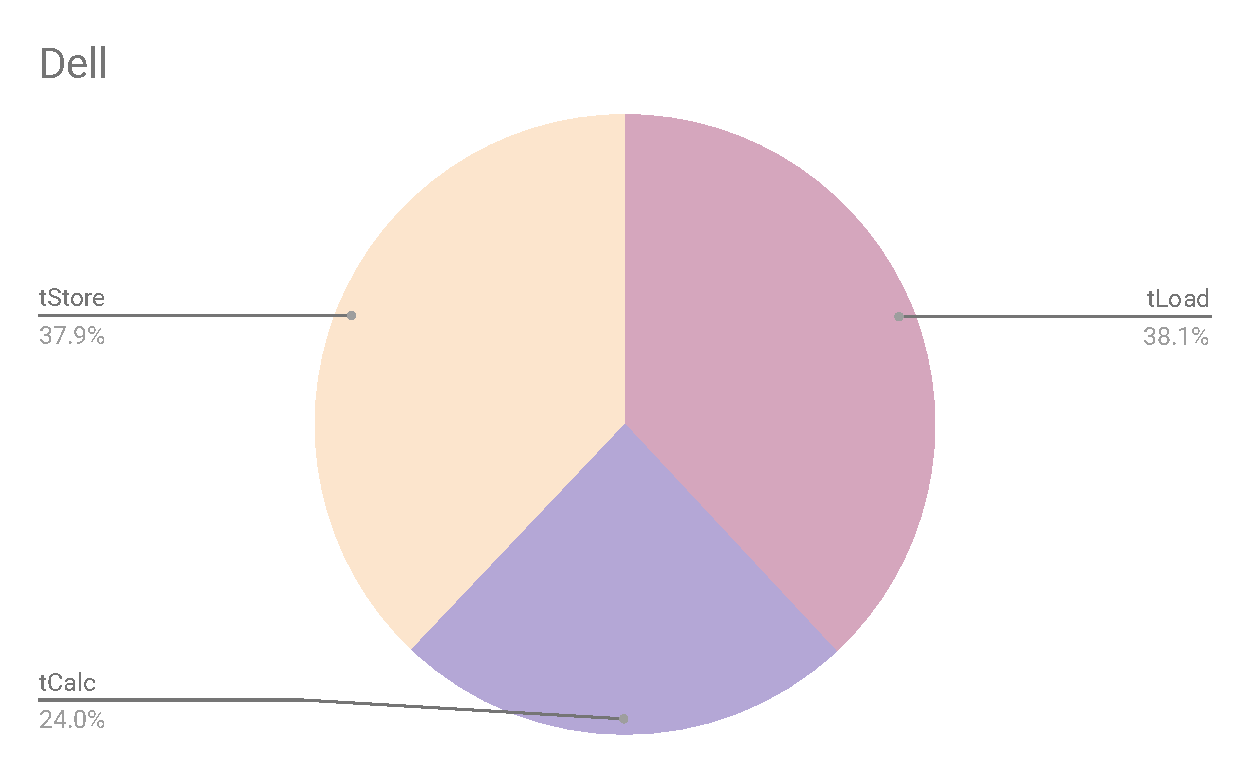
\includegraphics[width=0.45\textwidth]{Dell.pdf}
  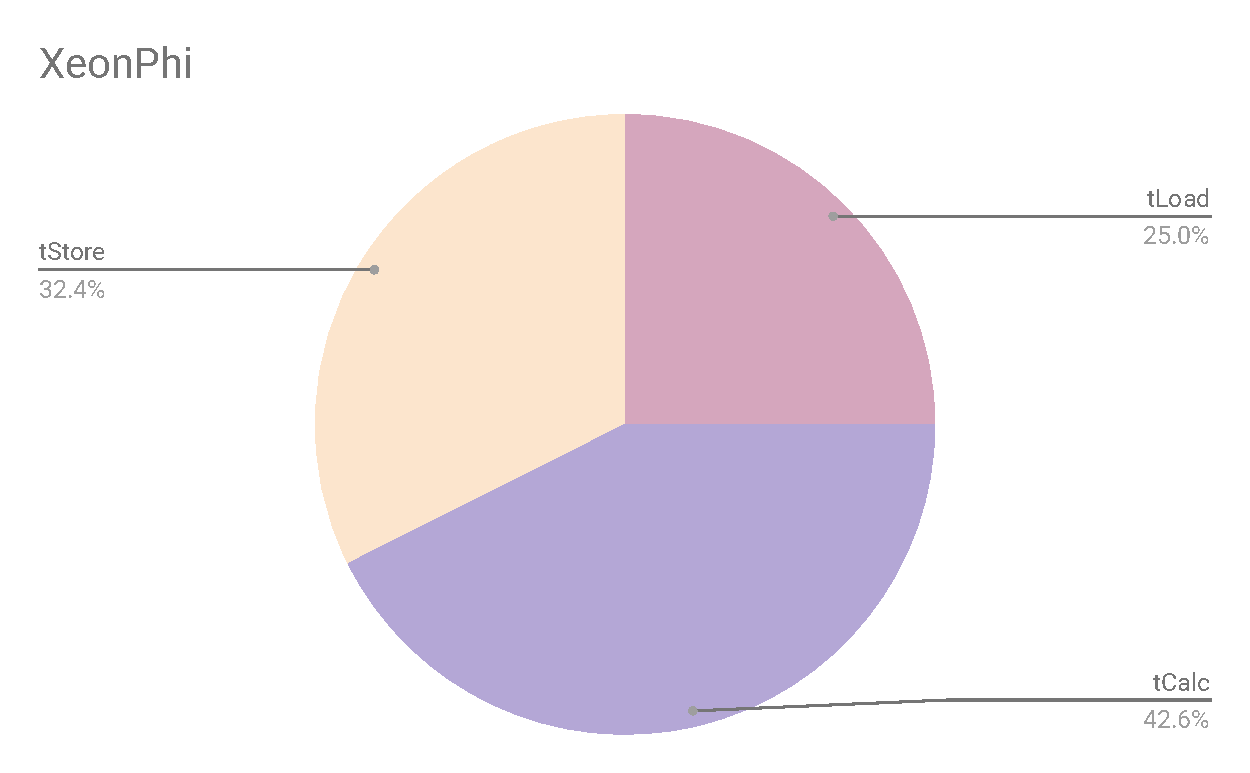
\includegraphics[width=0.45\textwidth]{XeonPhi.pdf}
  \caption{Percentage of time needed for loading an image, computing the watermark on it and storing the result}\label{fig:charts}
\end{figure}


As much as scalability is concerned, we can observe that the ``memory'' version of the watermarking problem allows more efficient implementations, as shown in \Cref{fig:scalability}. 

\begin{figure}[h]
  \centering
  \includegraphics[angle=270, width=0.85\textwidth]{scalability.eps}
  \vspace{1cm}
  \caption{Scalability of all the implemented parallel strategies on the watermark random85 on the Xeon Phi machine.}\label{fig:scalability}
\end{figure}


Moreover, another kind of otimization was performed in order to better exploit the characteristics of the Xeon Phi machine. We compiled all the programs (except for grPPi) using the Intel compiler \texttt{icc}. The results are shown in \Cref{fig:scalability_icc}

\begin{figure}[h]
  \centering
  \includegraphics[angle=270, width=0.85\textwidth]{scalabilityicc.eps}
  \vspace{1cm}
  \caption{Scalability of all the implemented parallel strategies compiled using icc and run on the watermark random85 on the Xeon Phi machine.}\label{fig:scalability_icc}
\end{figure}


%%%%%%%%%%%%%%~~~~~~~~~~~~~~~~~~~~~~~~~~~~~~~~~~~~~~~~%%%%%%%%%%%%%%%
\section{Conclusions}\label{end}

We can reasonably assert that the watermarking problem as stated in the Introduction cannot scale because of its intrinsics characteristics. On the other hand, the modified version of the problem which overcomes the issue of sequential I/Os does allow good scalability and speedup.

The best algorithms are both the data parallel strategy implemented via C++ threads and the stream parallel strategy, obtained through grPPi.

Furthermore, we may observe that in terms of programmability C++ threads require fewer lines of code, hence they may be preferrable in a certain sense.

\end{document}
